\documentclass{amsart}
\usepackage{amssymb,enumerate,bbm,amsmath}
\usepackage[colorlinks=true,linkcolor=blue,citecolor=blue]{hyper ref}
\usepackage{tikz}

\begin{document}

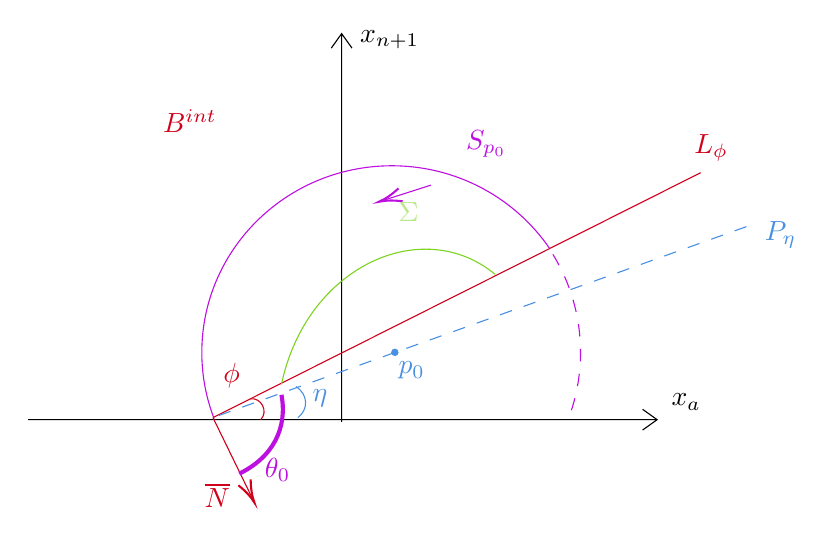
\begin{tikzpicture}[x=0.75pt,y=0.75pt,yscale=-1,xscale=1]
				
				\draw  (147.3,217) -- (450.3,217)(298.3,31) -- (298.3,218) (443.3,212) -- (450.3,217) -- (443.3,222) (293.3,38) -- (298.3,31) -- (303.3,38)  ;
				\draw [color={rgb, 255:red, 208; green, 2; blue, 27 }  ,draw opacity=1 ]   (471.3,98) -- (236.3,216) ;
				\draw [color={rgb, 255:red, 208; green, 2; blue, 27 }  ,draw opacity=1 ]   (254.3,207) .. controls (259.3,206) and (263.3,213) .. (259.3,217) ;
				\draw [color={rgb, 255:red, 74; green, 144; blue, 226 }  ,draw opacity=1 ] [dash pattern={on 4.5pt off 4.5pt}]  (493.3,124) -- (236.3,216) ;
				\draw  [draw opacity=0] (236.84,216.42) .. controls (233.09,206.72) and (231.01,196.21) .. (230.93,185.22) .. controls (230.57,135.58) and (271.24,95.04) .. (321.79,94.67) .. controls (353.83,94.44) and (382.14,110.4) .. (398.67,134.77) -- (322.44,184.55) -- cycle ; \draw  [color={rgb, 255:red, 189; green, 16; blue, 224 }  ,draw opacity=1 ] (236.84,216.42) .. controls (233.09,206.72) and (231.01,196.21) .. (230.93,185.22) .. controls (230.57,135.58) and (271.24,95.04) .. (321.79,94.67) .. controls (353.83,94.44) and (382.14,110.4) .. (398.67,134.77) ;  
				\draw  [draw opacity=0][dash pattern={on 4.5pt off 4.5pt}] (400.08,137.37) .. controls (408.4,150.88) and (413.26,166.81) .. (413.38,183.91) .. controls (413.47,195.86) and (411.24,207.28) .. (407.11,217.73) -- (325.44,184.55) -- cycle ; \draw  [color={rgb, 255:red, 189; green, 16; blue, 224 }  ,draw opacity=1 ][dash pattern={on 4.5pt off 4.5pt}] (400.08,137.37) .. controls (408.4,150.88) and (413.26,166.81) .. (413.38,183.91) .. controls (413.47,195.86) and (411.24,207.28) .. (407.11,217.73) ;  
				\draw [color={rgb, 255:red, 126; green, 211; blue, 33 }  ,draw opacity=1 ]   (269.3,200) .. controls (281.3,143) and (337.3,118) .. (372.3,147) ;
				\draw [color={rgb, 255:red, 189; green, 16; blue, 224 }  ,draw opacity=1 ]   (341.3,104) -- (318.2,111.39) ;
				\draw [shift={(316.3,112)}, rotate = 342.26] [color={rgb, 255:red, 189; green, 16; blue, 224 }  ,draw opacity=1 ][line width=0.75]    (10.93,-3.29) .. controls (6.95,-1.4) and (3.31,-0.3) .. (0,0) .. controls (3.31,0.3) and (6.95,1.4) .. (10.93,3.29)   ;
				\draw [color={rgb, 255:red, 74; green, 144; blue, 226 }  ,draw opacity=1 ]   (276.3,201) .. controls (282.3,205) and (282.3,212) .. (277.3,216) ;
				\draw [color={rgb, 255:red, 208; green, 2; blue, 27 }  ,draw opacity=1 ]   (236.3,216) -- (255.42,255.2) ;
				\draw [shift={(256.3,257)}, rotate = 244] [color={rgb, 255:red, 208; green, 2; blue, 27 }  ,draw opacity=1 ][line width=0.75]    (10.93,-3.29) .. controls (6.95,-1.4) and (3.31,-0.3) .. (0,0) .. controls (3.31,0.3) and (6.95,1.4) .. (10.93,3.29)   ;
				\draw  [color={rgb, 255:red, 74; green, 144; blue, 226 }  ,draw opacity=1 ][fill={rgb, 255:red, 74; green, 144; blue, 226 }  ,fill opacity=1 ] (322.44,184.55) .. controls (322.44,183.72) and (323.12,183.05) .. (323.94,183.05) .. controls (324.77,183.05) and (325.44,183.72) .. (325.44,184.55) .. controls (325.44,185.38) and (324.77,186.05) .. (323.94,186.05) .. controls (323.12,186.05) and (322.44,185.38) .. (322.44,184.55) -- cycle ;
				\draw [color={rgb, 255:red, 189; green, 16; blue, 224 }  ,draw opacity=1 ][line width=1.5]    (269.3,205) .. controls (272.3,221) and (265.3,235) .. (249,243) ;
				
				% Text Node
				\draw (166,143) node [anchor=north west][inner sep=0.75pt]   [align=left] {$ $};
				% Text Node
				\draw (306,28.4) node [anchor=north west][inner sep=0.75pt]    {$x_{n+1}$};
				% Text Node
				\draw (456,203.4) node [anchor=north west][inner sep=0.75pt]    {$x_{a}$};
				% Text Node
				\draw (240,188.4) node [anchor=north west][inner sep=0.75pt]  [color={rgb, 255:red, 208; green, 2; blue, 27 }  ,opacity=1 ]  {$\phi $};
				% Text Node
				\draw (211,66.4) node [anchor=north west][inner sep=0.75pt]  [color={rgb, 255:red, 208; green, 2; blue, 27 }  ,opacity=1 ]  {$B^{int}$};
				% Text Node
				\draw (324.44,111.08) node [anchor=north west][inner sep=0.75pt]  [color={rgb, 255:red, 126; green, 211; blue, 33 }  ,opacity=1 ] [align=left] {$\displaystyle \textcolor[rgb]{0.72,0.91,0.53}{\Sigma }$};
				% Text Node
				\draw (283,201.4) node [anchor=north west][inner sep=0.75pt]  [color={rgb, 255:red, 74; green, 144; blue, 226 }  ,opacity=1 ]  {$\eta $};
				% Text Node
				\draw (231,246.4) node [anchor=north west][inner sep=0.75pt]  [color={rgb, 255:red, 208; green, 2; blue, 27 }  ,opacity=1 ]  {$\overline{N}$};
				% Text Node
				\draw (260,234.4) node [anchor=north west][inner sep=0.75pt]  [color={rgb, 255:red, 189; green, 16; blue, 224 }  ,opacity=1 ]  {$\theta _{0}$};
				% Text Node
				\draw (501,120.4) node [anchor=north west][inner sep=0.75pt]  [color={rgb, 255:red, 74; green, 144; blue, 226 }  ,opacity=1 ]  {$P_{\eta }$};
				% Text Node
				\draw (467,78.4) node [anchor=north west][inner sep=0.75pt]  [color={rgb, 255:red, 208; green, 2; blue, 27 }  ,opacity=1 ]  {$L_{\phi }$};
				% Text Node
				\draw (324.44,187.95) node [anchor=north west][inner sep=0.75pt]  [color={rgb, 255:red, 74; green, 144; blue, 226 }  ,opacity=1 ]  {$p_{0}$};
				% Text Node
				\draw (357,76.4) node [anchor=north west][inner sep=0.75pt]  [color={rgb, 255:red, 189; green, 16; blue, 224 }  ,opacity=1 ]  {$S_{p_{0}}$};
				
				
			\end{tikzpicture}

\end{document}